\documentclass{article}

\usepackage{changepage}
\usepackage{graphicx}
\usepackage{float}
\usepackage[export]{adjustbox}
\usepackage[toc,page]{appendix}
\usepackage[backend=biber, style=authoryear-icomp]{biblatex}

\addbibresource{~/Documents/latex_bibliography.bib}

\title{IN618 - Security Assignment 1: Security Audit Report for the Deathstar Server}
\author{Prepared by Matthew Hall}
\date{}

\begin{document}
\pagenumbering{gobble}
\maketitle
\renewcommand{\abstractname}{Executive Summary}
\begin{abstract}	
This document summarises the findings from an independent security audit commissioned by the Rebel Alliance to investigate the Death Star server.
A total of three security vulnerabilities were discovered and exploited successfully along with numerous unexploited vulnerabilities.
All three of these exploits can be used to great effect to gain unauthorized access to the target server.
One of these granted a remote shell as the root user.
Nine out of ten requested pieces of intelligence were recovered.
The system's password file was extracted and all user passwords, in one way or another, were cracked.

Recommendations to improve security include ensuring the patching of out-of-date software, implementing a firewall, investigating for rogue employees, implementing a strict password policy, redesigning a web app hosted on the server and the encryption of sensitive information.
\end{abstract}
\newpage
\pagenumbering{arabic}

\tableofcontents
\newpage

\section{Network Information}
\label{sec:network_information}

\subsection{Discovering hosts with nmap}
\label{subsec:discovering_hosts}
\paragraph{}
I used the following commands during the host discovery process:
\begin{adjustwidth}{-1cm}{}
\begin{verbatim}
# identifies hosts with IP addresses in the network space of 192.168.100.0/24
nmap -sn 192.168.100.1
# attempts to identify the operating system of the host with address 192.168.100.1
nmap -O 192.168.100.1
# attempts to identify the operating system of the host with address 192.168.100.115
nmap -O 192.168.100.115
# attempts to identify the operating system of the host with address 192.168.100.253
nmap -O 192.168.100.253
\end{verbatim}
\end{adjustwidth}

\subsection{Network Diagram}
\label{subsec:network_diagram}
\begin{figure}[h!]
	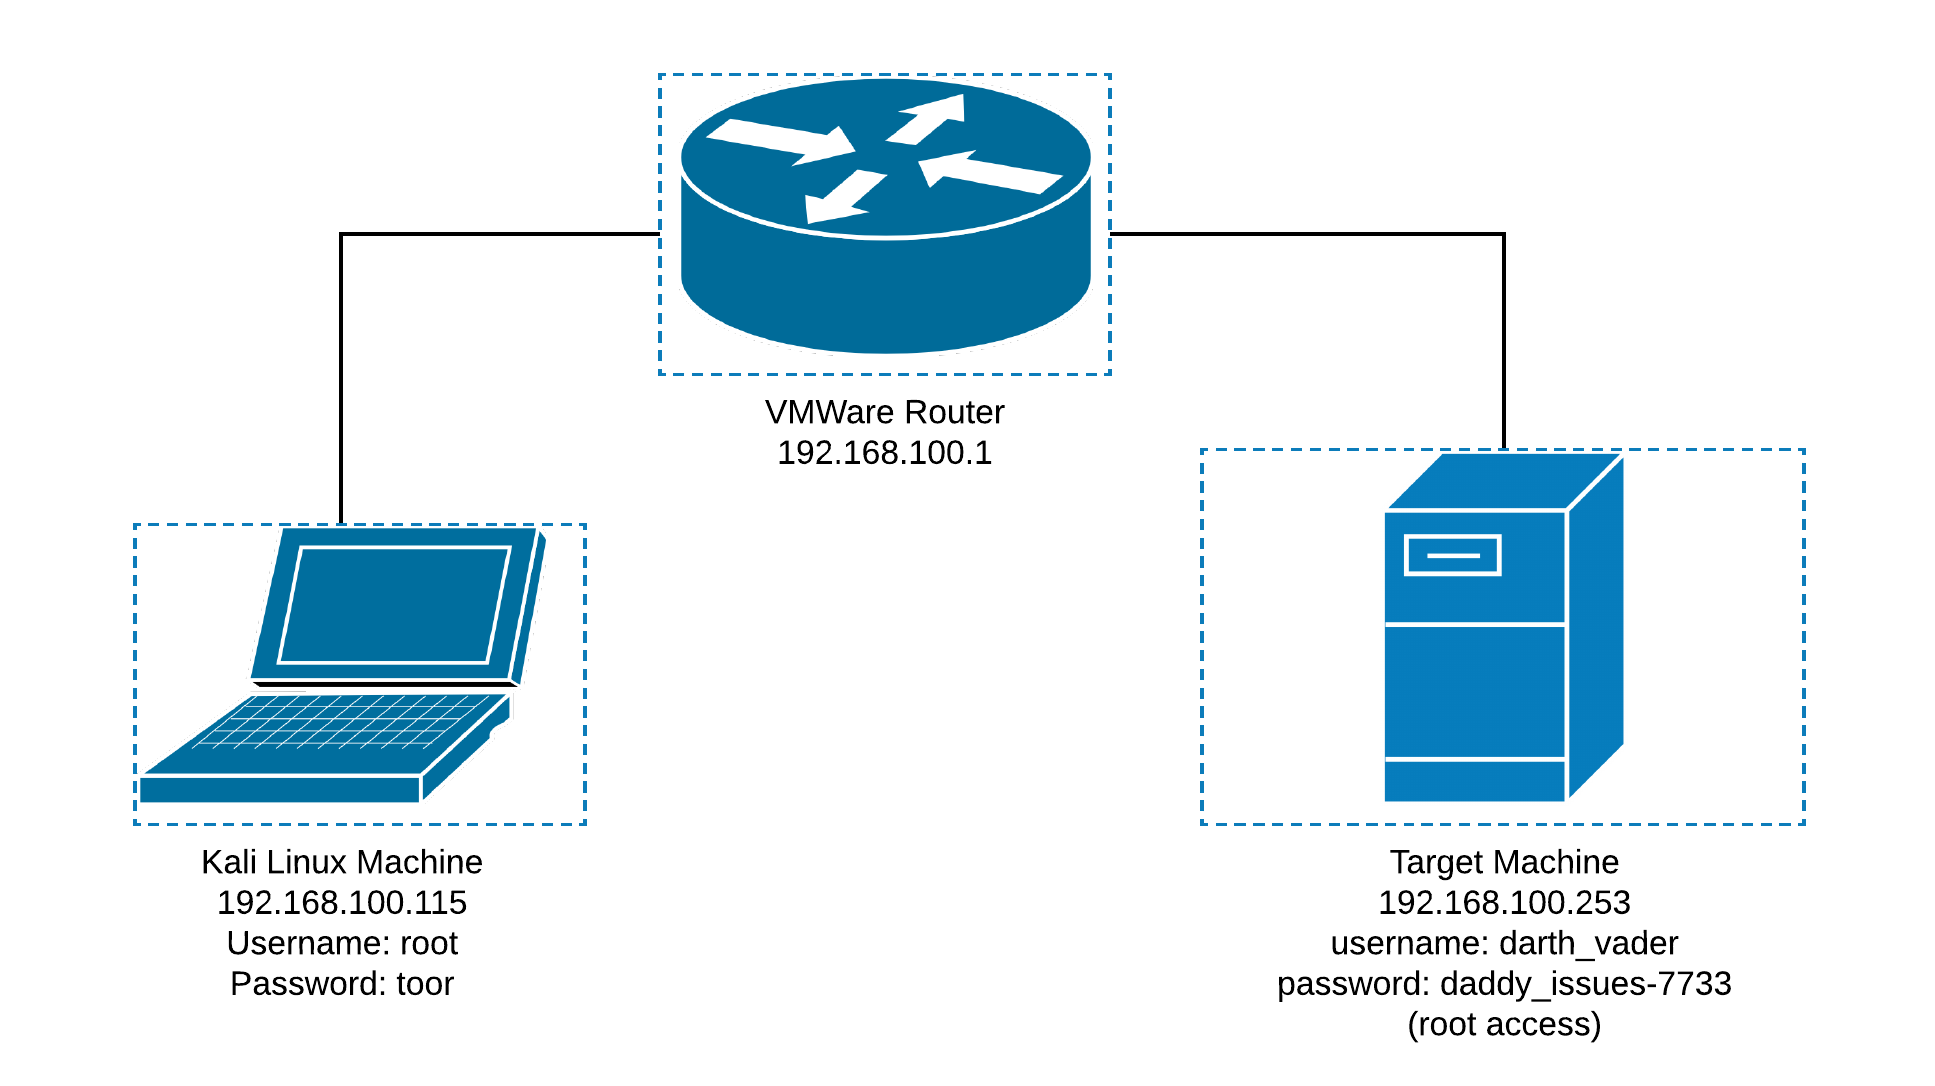
\includegraphics[width=\linewidth]{resources/network-diagram-new.png}
	\caption{Network diagram of address space \texttt{192.168.100.0/24}}
	\label{fig:network_diagram}
\end{figure}

\subsection{Target Machine Information}
\label{subsec:target_info}
\paragraph{}
\begin{itemize}
	\item \textbf{Target hostname}: \texttt{death-star}
	\item \textbf{Target IP address}: \texttt{192.168.100.253}
	\item \textbf{Target MAC address}: \texttt{00:50:56:86:F2:31}
	\item \textbf{Target MAC vendor}: \texttt{VMWare}
	\item \textbf{Operating System version}: \texttt{Ubuntu 14.04.01 LTS "Trusty Tahr"}
	\item \textbf{Linux Kernel version}: \texttt{3.13}
\end{itemize}

\newpage

\section{Open Ports and Running Services}
\label{sec:services}
\paragraph{}
By use of the nmap command \texttt{nmap -sV 192.168.100.253}, I was able to retrieve the following information about what services on the target machine are running on what ports:
\newline
\newline

\begin{adjustwidth}{-2cm}{}
\begin{tabular}{ |c|c|c|l| }
\hline
Port Number & State & Service & Version \\
\hline
21/tcp & open & ftp & ProFTPD 1.3.5 \\
\hline
22/tcp & open & ssh & OpenSSH 6.6.1p1 Ubuntu 2ubuntu2.10 (Ubuntu Linux; protocol 2.0) \\
\hline
80/tcp & open & http & Apache httpd 2.4.7 \\
\hline
111/tcp & open & rpcbind & 2-4 (RPC \# 100000) \\
\hline
139/tcp & open & netbios-ssn & Samba smbd 3.X - 4.X (workgroup: WORKGROUP) \\
\hline
445/tcp & open & netbios-ssn & Samba smbd 3.X - 4.X (workgroup: WORKGROUP) \\
\hline
3306/tcp & open & mysql & MySQL (unauthorized) \\
\hline
6667/tcp & open & irc & UnrealIRCd \\
\hline
6697/tcp & open & irc & UnrealIRCd \\
\hline
8067/tcp & open & irc & UnrealIRCd \\
\hline
8080/tcp & open & http & Jetty 8.1.7.v20120910 \\
\hline
8181/tcp & open & http & WEBrick httpd 1.3.1 (Ruby 2.3.6 (2017-12-14)) \\
\hline
49307/tcp & open & status & 1 (RPC \# 100024) \\
\hline
\end{tabular}
\end{adjustwidth}

\newpage

\section{Vulnerability Identification}
\label{sec:vulnerability_identification}
\paragraph{}
The following services on the target machine had exploitable vulnerabilities:

% Port 21/tcp
\subsection{ProFTPD 1.3.5 (port 21/tcp)}
\label{subsec:pro_ftpd}
\paragraph{}
Version 1.3.5 of ProFTPD has vulnerability \emph{CVE-2015-3306}, which allows attackers to read and write to arbitrary files via the \texttt{site cpfr} and \texttt{site cpto} commands \parencite{mitre20153306}.
Metasploit has the module \texttt{exploit/unix/ftp/proftpd\_modcopy\_exec} which exploits this flaw.
By using this module and specifying the \texttt{SITEPATH} option to be \texttt{/var/www/html}, I was able to remotely log in to the machine as the \texttt{www-data} user.
While logged in, I was able to download files in the \texttt{/var/www/html} directory\footnote{Among those files was the administrator account details of the phpMyAdmin service} and traverse the rest of the filesystem after starting an interactive shell.

% Ports 6667/tcp, 6697/tcp and 8067/tcp
\subsection{UnrealIRCd 3.2.8.1 (port 6667/tcp)}
\label{subsec:unreal_ircd}
\paragraph{}
During the period of time from November 2009 to June 2010, version 3.2.8.1 of UnrealIRCd contained \emph{CVE-2010-2075}: a backdoor allowing remote attackers to login to the system and execute arbitrary commands.\footnote{https://cve.mitre.org/cgi-bin/cvename.cgi?name=CVE-2010-2075}
This vulnerability was only present in copies of the software downloaded from particular mirror sites.
This backdoor, if present, can be exploited with metasploit module \texttt{exploit/unix/irc/unreal\_irc\_3281\_backdoor}.
Using this exploit, I was able to remotely log in to the machine as the \texttt{boba\_fett} user\footnote{This user had a text file in their home directory containing the login information for the \texttt{darth\_vader} user.} and use the machine as if I were in an ssh session, all without having to supply a password.

% Port 8080/tcp
\subsection{Apache Continuum 1.4.2 (port 8080/tcp)}
\label{subsec:apache_continuum}
\paragraph{}
The server was hosting the Jetty web server (verison 8.1.7v20120910) on port 8080, which was running Apache Continuum 1.4.2.
This version of Continuum has vulnerability \emph{EDB-39886}, which allows attackers to perform arbitrary code injection\footnote{https://www.exploit-db.com/exploits/39886}.
I was able to exploit this using the metasploit module \texttt{exploit/linux/http/apache\_continuum\_cmd\_exec}.
Using this exploit, I was granted root access to the machine and was able to read and download root-only files, including the \texttt{/etc/shadow} file as well as the server's private ssh keys.
I was able to do all of this without supplying a password.

\newpage

\section{Information Extraction}
\label{sec:info_extraction}
\paragraph{}
As requested, I have located and extracted both the login details of every user account on the system and all information regarding the plans of the Galactic Empire.

\subsection{Login Details}
\label{subsec:login_details}
\begin{adjustwidth}{-1.5cm}{}
\begin{tabular}{ |c|c|c|c| }
\hline
\textbf{Username} & \textbf{Password} & \textbf{Password Hash (md5crypt)} & \textbf{Password Salt} \\
\hline
storm\_trooper\_1 & starwarsrocks & \texttt{HmlEMwzAUCz0NEitMjx9d1} & \texttt{lnwk829Q} \\
\hline
storm\_trooper\_2 & stormtrooper1 & \texttt{7a/Tj3TjRzZYR6mhbZksq0} & \texttt{9AJdbBeI} \\
\hline
storm\_trooper\_3 & Lego starwars & \texttt{N7hkGMUGsyeBgNPwIaF/40} & \texttt{WdB.ds.7} \\
\hline
storm\_trooper\_4 & starwarsbatman & \texttt{5F/sLNVjUPMFtLUdS.hog.} & \texttt{.jX4bdHx} \\
\hline
storm\_trooper\_5 & Password1234567 & \texttt{w6VyqglDCJot.Xeb9slLI0} & \texttt{0HHFKzl.} \\
\hline
imperial\_guards & starwars4life & \texttt{ebSf18qOk7tgu.iMqf.bi/} & \texttt{v9GI28ar} \\
\hline
captain\_needa & \emph{darksidegod@hotmail.com} & \texttt{FO9c2OF4Qf1onEyYkq.gK/} & \texttt{VtXabEV0} \\
\hline
admiral\_piett & darksideofthemoon & \texttt{cTG0isRNogwyCeQwCZJXF.} & \texttt{D06DmZeK} \\
\hline
admiral\_ozzel & darksiderules & \texttt{eFPtaxBv7sX5IDp8Bc19h.} & \texttt{lfbtu2co} \\
\hline
general\_veers & darkside3000@hotmail.com & \texttt{AJlGTM7XYFaY3Ezr7Av/u/} & \texttt{.wG8JtvN} \\
\hline
emperor\_palpatine & 912Deathstars & \texttt{hy9v3MmcpwRq/G3Dhtu2U1} & \texttt{Sr5iUN.o} \\
\hline
darth\_sidious & 7ujMko0admin & \texttt{Mp7O4bzX8bmWsGGV8ZrVY0} & \texttt{TyPfW4pp} \\
\hline
boba\_fett & \emph{bountyhunter1976} & \texttt{GfHV875pepnKEg.JC.zYY/} & \texttt{eOF0T0eZ} \\
\hline
death\_star\_admin & \textless 3DeathStars\textless 3 & \texttt{erKQWB6ZTfw2efmZMPDME.} & \texttt{HnIyNzWr} \\
\hline
darth\_vader & \emph{daddy\_issues-7733} & \texttt{0TkhYTZFnI1srHEzG1TrO/} & \texttt{AnAm41bc} \\
\hline
\end{tabular}
\end{adjustwidth}

\paragraph{}
The plaintext passwords that are written in italics were found in plaintext form (see section~\ref{subsec:bad_passwords}).
The others were found in their salted md5crypt form and were recovered with hashcat using the rockyou dictionary and the \texttt{default\_pass\_for\_services\_unhash} dictionary included in Metasploit.

\newpage

\subsection{Plans of the Empire}
\label{subsec:empire_plans}
\paragraph{}
In order to locate the requested intelligence files, I used the following command:
\begin{verbatim}
root@deathstar:/# locate -i --regex '(death|rebel)[_-]?(star|alliance)'
\end{verbatim}
Below are the names and locations of the extracted intelligence files. The contents of the files can be found in the Intelligence Appendix (Appendix~\ref{appendix:intelligence}).

\paragraph{}
In the directory \texttt{/home/death\_star\_admin/death-star\_plans}:
\begin{itemize}
	\item \texttt{deathstar-crafts.png}, Figure~\ref{fig:deathstar_crafts}
	\item \texttt{deathstar-cross-section.png}, Figure~\ref{fig:deathstar_cross_section}
	\item \texttt{deathstar-operations.png}, Figure~\ref{fig:deathstar_operations}
	\item \texttt{deathstar-summary.png}, Figure~\ref{fig:deathstar_summary}
	\item \texttt{deathstar-techincal-specs-diagram.png}, Figure~\ref{fig:deathstar_technical_specs_diagram}
\end{itemize}

\paragraph{}
In the directory \texttt{/home/general\_veers/rebel-information}:
\begin{itemize}
	\item \texttt{rebel-alliance-fleet-1.jpg}, Figure~\ref{fig:rebel_alliance_fleet_1}
	\item \texttt{rebel-alliance-fleet-2.jpg}, Figure~\ref{fig:rebel_alliance_fleet_2}
\end{itemize}

\paragraph{}
In the directory \texttt{/home/darth\_sidious}:
\begin{itemize}
	\item \texttt{death-star-weakness.png}, Figure~\ref{fig:death_star_weakness}
\end{itemize}

\paragraph{}
In the directory \texttt{/home/darth\_vader}:
\begin{itemize}
	\item \texttt{i-love-my-death-star.jpg}, Figure~\ref{fig:i_love_my_death_star}
\end{itemize}

\paragraph{}
In the directory \texttt{/opt/proftpd/share/locale}
\begin{itemize}
	\item \texttt{deathstarinfographic.pNg}, Figure~\ref{fig:deathstarinfographic}
\end{itemize}

\newpage

\section{Security Recommendations}
\label{sec:security_recommendations}
\paragraph{}
Over the course of this audit, I have discovered multiple vulnerabilities in key services running on the Death Star server and exploited them.
I have also found many other security issues during my investigation of the server.
Here I have compiled the details of all of the security flaws I could find with this server, as well as various recommendations to fix these problems for the future.

% Ubuntu 14.04 LTS nearing end-of-life, upgrade to 18.04 LTS
\subsection{Upgrade Operating System}
\label{subsec:upgrade_os}
\paragraph{}
The operating system on the Death Star server was Ubuntu 14.04 LTS, which is due to stop receiving security updates in April 2019.
Because of this, it is imperative that the operating system is upgraded to a new version.

\paragraph{}
\begin{adjustwidth}{1.5cm}{1.5cm}
	Security recommendations regarding unsupported operating systems:
	\begin{enumerate}
		\item Upgrade to Ubuntu 18.04 LTS, which will receive security updates until 2023. Additionally, installations of Ubuntu can be upgraded to later releases easily via the command line by use of the \texttt{do-release-upgrade} command.
	\end{enumerate}
\end{adjustwidth}

% Unpatched software contains vulnerabilities
\subsection{Upgrade Software}
\label{subsec:upgrade_software}
\paragraph{}
Many of the services provided by the Death Star server were running outdated software that contained vulnerabilities.
Out-of-date software is much more likely to contain vulnerabilities than up-to-date versions.

\paragraph{}
\begin{adjustwidth}{1.5cm}{1.5cm}
	Security recommendations regarding out-of-date software:
	\begin{enumerate}
		\item Update your software. \emph{Now.}
	\end{enumerate}
\end{adjustwidth}

% No firewall / packet filtering - do that
\subsection{Firewall}
\label{subsec:firewall}
\paragraph{}
The Death Star server did not have any kind of firewall.
Because of this, an attacker could easily scan every port on the system and send malicious data packets to the server.

\paragraph{}
\begin{adjustwidth}{1.5cm}{1.5cm}
	Security recommendations regarding firewalls:
	\begin{enumerate}
		\item I would recommend the installation of a physical firewall, ideally running an OS designed for the purpose of being a firewall/router such as pfSense.
		\item If the budget does not allow this, some kind of packet-filtering process should be implemented on the server.
	\end{enumerate}
	I personally can vouch for the use of iptables, a software firewall that is available on virtually every Linux distribution.
\end{adjustwidth}
% darth_vader wrote script to sql-inject payroll app
\subsection{Inside Threats}
\label{subsec:inside_threats}
\paragraph{}
During my investigation, I found a questionable Ruby script in the \texttt{/home/darth\_vader} folder, implying that they were created by this user.
Upon analysing the contents of the file, it appears to perform an SQL injection attack on the Death Star's payroll app (see section~\ref{subsec:payroll_app}).
All of this implies that there is a rogue employee of the Empire using the Death Star server.

\paragraph{}
\begin{adjustwidth}{1.5cm}{1.5cm}
	Security recommendations regarding the possibility of a rogue employee:
	\begin{enumerate}
		\item \emph{This cannot be ignored and must be investigated as soon as possible.} 
	\end{enumerate}
\end{adjustwidth}

% /etc/shadow, MySQL, writing passwords down in plaintext
\subsection{Insecure Password Storage and Bad User Passwords}
\label{subsec:bad_passwords}
\paragraph{}
During my attempts to recover passwords, I was able to recover passwords in three different ways.

\paragraph{}
The first method I was able to use was simply reading a user's password that was written down in a file. Incidentally, this was the password of the \texttt{darth\_vader} user.
I was able to log in to the account with the password I found and created another account for myself in the process. I was able to do this because the \texttt{darth\_vader} user had superuser access.

\paragraph{}
The second method I was able to use to recover passwords was by exploiting the payroll app.
The payroll app on the Death Star server has numerous security issues (see section ~\ref{subsec:payroll_app}) and one of those issues was the fact that the user passwords were stored in plaintext.
I went through each password I found in the app and attempted to log in to the corresponding user account.
I was able to log in as the \texttt{captain\_needa} and \texttt{boba\_fett} users. Incidentally, the \texttt{boba\_fett} user was the user that had the password for \texttt{darth\_vader} in their home directory.

\paragraph{}
The third method I used\footnote{And expected to use} was password cracking. By using the \texttt{hashcat} tool I was able to crack the remaining user's passwords with two dictionary attacks (see section~\ref{subsec:login_details}).
Using a relatively powerful GPU\footnote{A GTX 1050ti} I successfully recovered the remaining passwords with roughly 20 minutes of computing time.
This is due to two problems with the password on the server.
The first problem is that the user's passwords were relatively common passwords, whether the users were aware of this or not.
The second problem is that the passwords were hashed+salted using md5crypt.
This hashing algorithm is too fast to be used for storing passwords and should not have been used on the server.
This is a problem because if a hashing algorithm is too fast, it becomes easy for attackers to guess what a hashed password might be.

\paragraph{}
\begin{adjustwidth}{1.5cm}{1.5cm}
	Security recommendations regarding passwords and password storage:
	\begin{enumerate}
		\item \emph{ALL EMPLOYEES MUST CHANGE ALL OF THEIR PASSWORDS IMMEDIATELY}
		\item All employees must be educated about
		\begin{enumerate}
			\item The dangers of using easy-to-guess passwords
			\item The dangers of storing/writing down passwords in plaintext
			\item The dangers of reusing passwords
			\item How to think of good passwords (see below for example method)
		\end{enumerate}
		\item Future passwords should be stored by salting and hashing using a secure, trusted cryptographic hashing algorithm (see below)
		\item The owner of the \texttt{boba\_fett} user should be sentenced to death by sarlacc
	\end{enumerate}
\end{adjustwidth}

\paragraph{}
A reasonable technique for making a password is as follows:
\begin{enumerate}
	\item Choose three random, 8-10 letter words
	\item Choose another reasonably long, more obscure word (or even a made-up word)
	\item Pick a symbol and put it between two of the words
\end{enumerate}
As for hashing, I would recommend using the SHA-512 algorithm instead of md5crypt, since SHA-512 is slower (and therefore harder to guess a hashed password) and practically impossible\footnote{At the time of writing} to generate a collision with this algorithm.

% Payroll app is insecure
\subsection{Poorly Designed Payroll App}
\label{subsec:payroll_app}
\paragraph{}
The payroll app on the server is incredibly insecure and needs to be replaced as soon as possible.
Firstly, the source code contains the password for the \texttt{root} account on the MySQL server.
This means that anyone on the server can view the source code, read the password and log in as the root user.
This can be remedied by changing the file permissions so that only the root user can view the contents of the file.

\paragraph{}
Secondly, the app is vulnerable to SQL injection to the extent that I was able to print arbitrary information from the database to the screen via the username input box.
The input that I used to extract the following data was:
\begin{verbatim}
' UNION(SELECT username,password,3,4 FROM payroll.users);--
\end{verbatim}
\begin{figure}[H]
	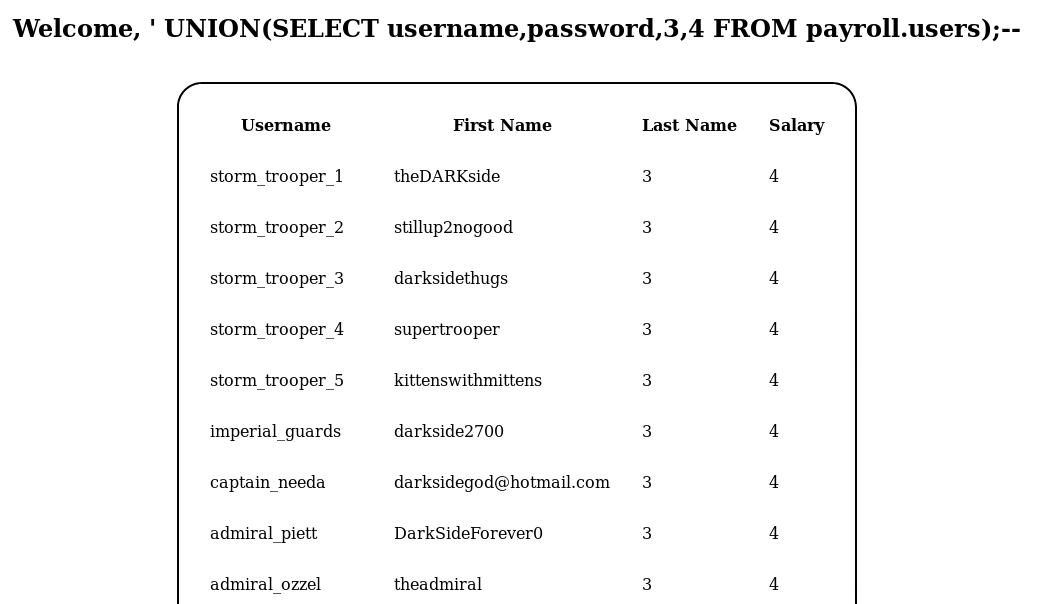
\includegraphics[width=\linewidth, frame]{resources/sql_injection.png}
	\caption{Results from SQL injection}
	\label{fig:sql_injection}
\end{figure}
This can be fixed by changing the app's code to use prepared statements, which are currently considered the safe way to interact with a database via a web form.

\paragraph{}
Finally, as you may have deduced from the screenshot above (figure~\ref{fig:sql_injection}), the app stores the user's passwords in plaintext.
This is incredibly bad practice for a number of reasons.
For one, users tend to reuse the same password for multiple services\footnote{Even though they shouldn't} (see section~\ref{subsec:bad_passwords}), which means an attacker can find passwords on insecure websites and login on other websites using the same username and password combination.
Also, a rogue insider (which you may have, section~\ref{subsec:inside_threats}) with access to the database can gain access much more easily than an outside attacker, meaning they can steal the passwords of everyone using the app.
Additionally, should you offer the ability for a user to click a 'I forgot my password' button and send them their password via email, the email could be intercepted and the password stolen that way.

\paragraph{}
\begin{adjustwidth}{1.5cm}{1.5cm}
	Security recommendations regarding the payroll app:
	\begin{enumerate}
		\item \emph{ALL EMPLOYEES MUST CHANGE ALL OF THEIR PASSWORDS IMMEDIATELY}
		\item The payroll app must be re-programmed to use prepared statements
		\item The app should use a separate authentication service, such as OAuth to handle logging in
		\item If the above is not possible, future passwords must be stored by salting and hashing with a modern, trusted cryptographic hashing algorithm (see recommendations in section~\ref{subsec:bad_passwords})
	\end{enumerate}
\end{adjustwidth}

% Sensitive information was not encrypted
\subsection{Sensitive Information}
\label{subsec:sensitive_info}
\paragraph{}
I found it relatively easy to locate the pieces of intelligence I was tasked with finding.
Unfortunately for the Empire, I also found the intelligence easy to read.
What I mean by this is that these files has no special protections in place to prevent them from being read by those who are not meant to read them.

\paragraph{}
\begin{adjustwidth}{1.5cm}{1.5cm}
	Security recommendations regarding the storing of sensitive information:
	\begin{enumerate}
		\item Encrypt the files with an encryption tool such as PGP.
	\end{enumerate}
\end{adjustwidth}
\newpage

\section{Conclusions}
\label{sec:conclusions}
\paragraph{}
This document summarised the findings from an independent security audit commissioned by the Rebel Alliance to investigate the Death Star server.
A total of three security vulnerabilities were discovered and exploited successfully root access was acquired.
This is an incredibly insecure server and drastic measures would need to be taken to mitigate the security risks present and secure the sensitive information stored on the system.
The security recommendations given in this report should be applied to the machines of the Rebel Alliance and then another security audit should be performed to re-asses the security of their servers.

\newpage
\printbibliography
\newpage

\begin{appendices}
\section{Intelligence Appendix}
\label{appendix:intelligence}

\begin{figure}[H]
	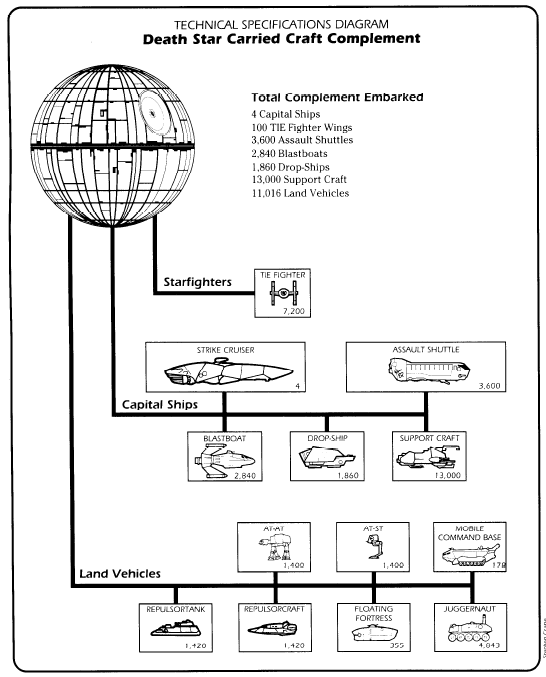
\includegraphics[width=\linewidth]{resources/plans/deathstar-crafts.png}
	\caption{\texttt{deathstar-crafts.png}}
	\label{fig:deathstar_crafts}
\end{figure}

\begin{figure}[H]
	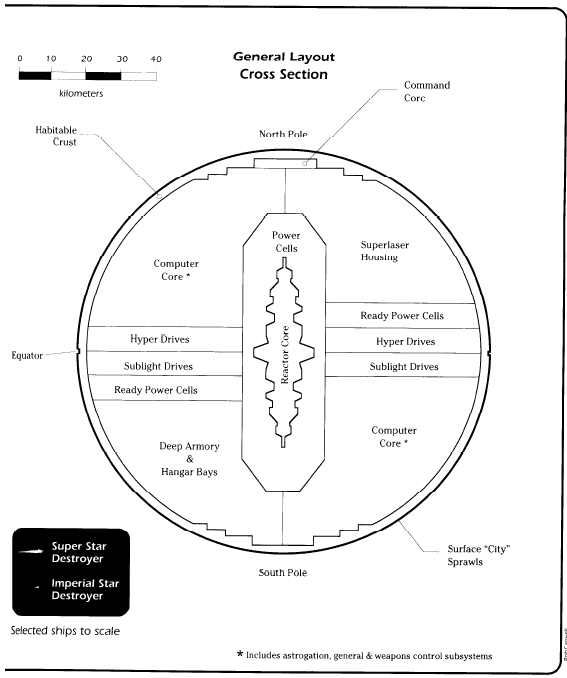
\includegraphics[width=\linewidth]{resources/plans/deathstar-cross-section.png}
	\caption{\texttt{deathstar-cross-section.png}}
	\label{fig:deathstar_cross_section}
\end{figure}

\begin{figure}[H]
	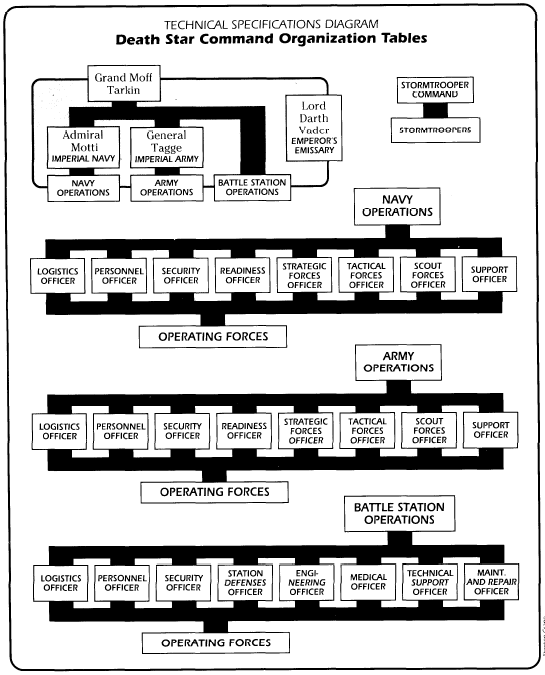
\includegraphics[width=\linewidth]{resources/plans/deathstar-operations.png}
	\caption{\texttt{deathstar-operations.png}}
	\label{fig:deathstar_operations}
\end{figure}

\begin{figure}[H]
	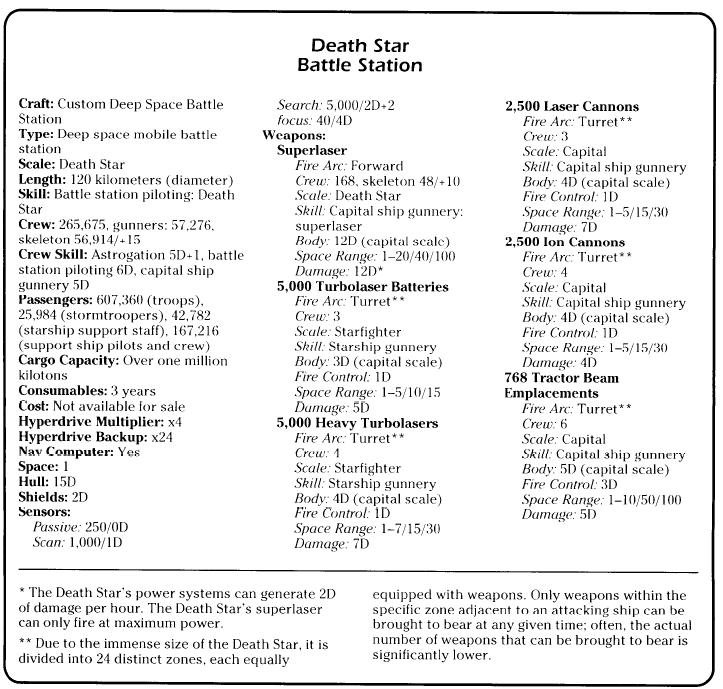
\includegraphics[width=\linewidth]{resources/plans/deathstar-summary.png}
	\caption{\texttt{deathstar-summary.png}}
	\label{fig:deathstar_summary}
\end{figure}

\begin{figure}[H]
	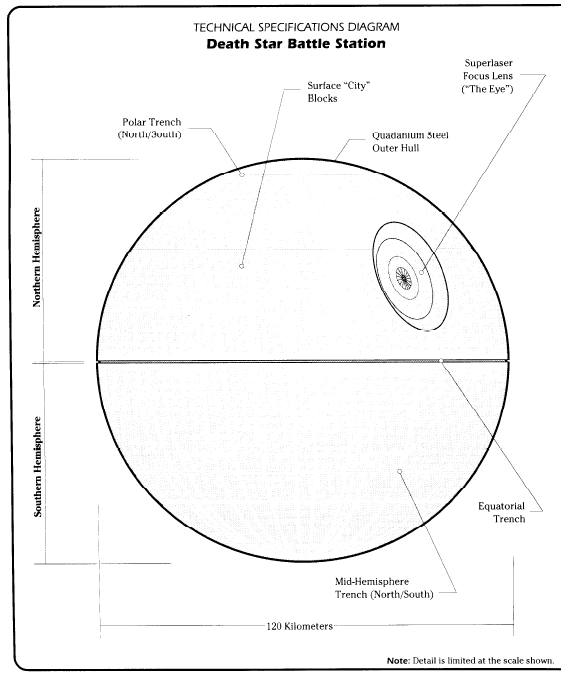
\includegraphics[width=\linewidth]{resources/plans/deathstar-technical-specs-diagram.png}
	\caption{\texttt{deathstar-techincal-specs-diagram.png}}
	\label{fig:deathstar_technical_specs_diagram}
\end{figure}

\begin{figure}[H]
	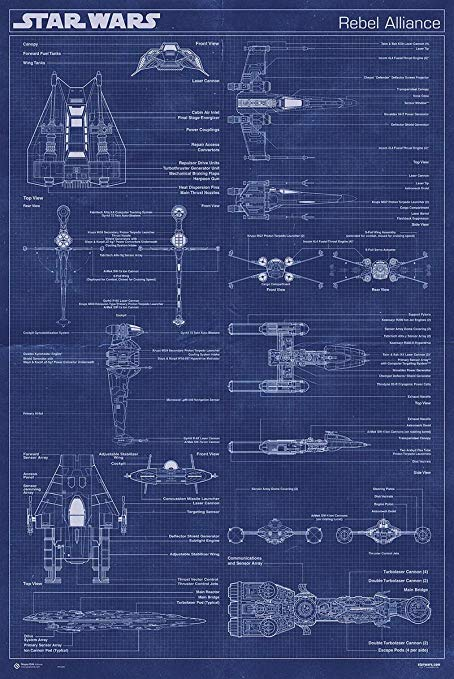
\includegraphics[width=\linewidth]{resources/plans/rebel-alliance-fleet-1.jpg}
	\caption{\texttt{rebel-alliance-fleet-1.jpg}}
	\label{fig:rebel_alliance_fleet_1}
\end{figure}

\begin{figure}[H]
	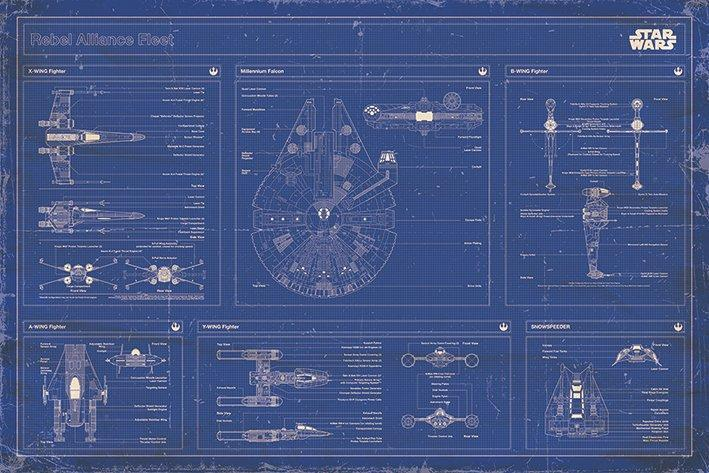
\includegraphics[width=\linewidth]{resources/plans/rebel-alliance-fleet-2.jpg}
	\caption{\texttt{rebel-alliance-fleet-2.jpg}}
	\label{fig:rebel_alliance_fleet_2}
\end{figure}

\begin{figure}[H]
	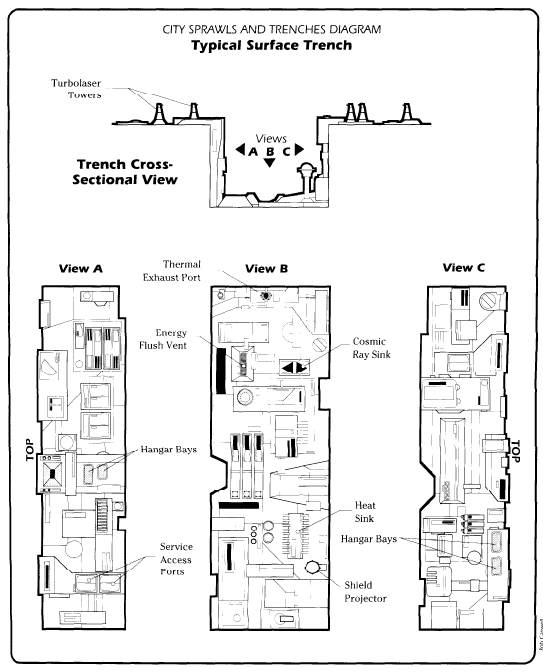
\includegraphics[width=\linewidth]{resources/plans/death-star-weakness.png}
	\caption{\texttt{death-star-weakness.png}}
	\label{fig:death_star_weakness}
\end{figure}

\begin{figure}[H]
	
\includegraphics[width=\linewidth]{resources/plans/i-love-my-death-star.jpg}
	\caption{\texttt{i-love-my-death-star.jpg}}
	\label{fig:i_love_my_death_star}
\end{figure}

%\begin{figure}[H]
%	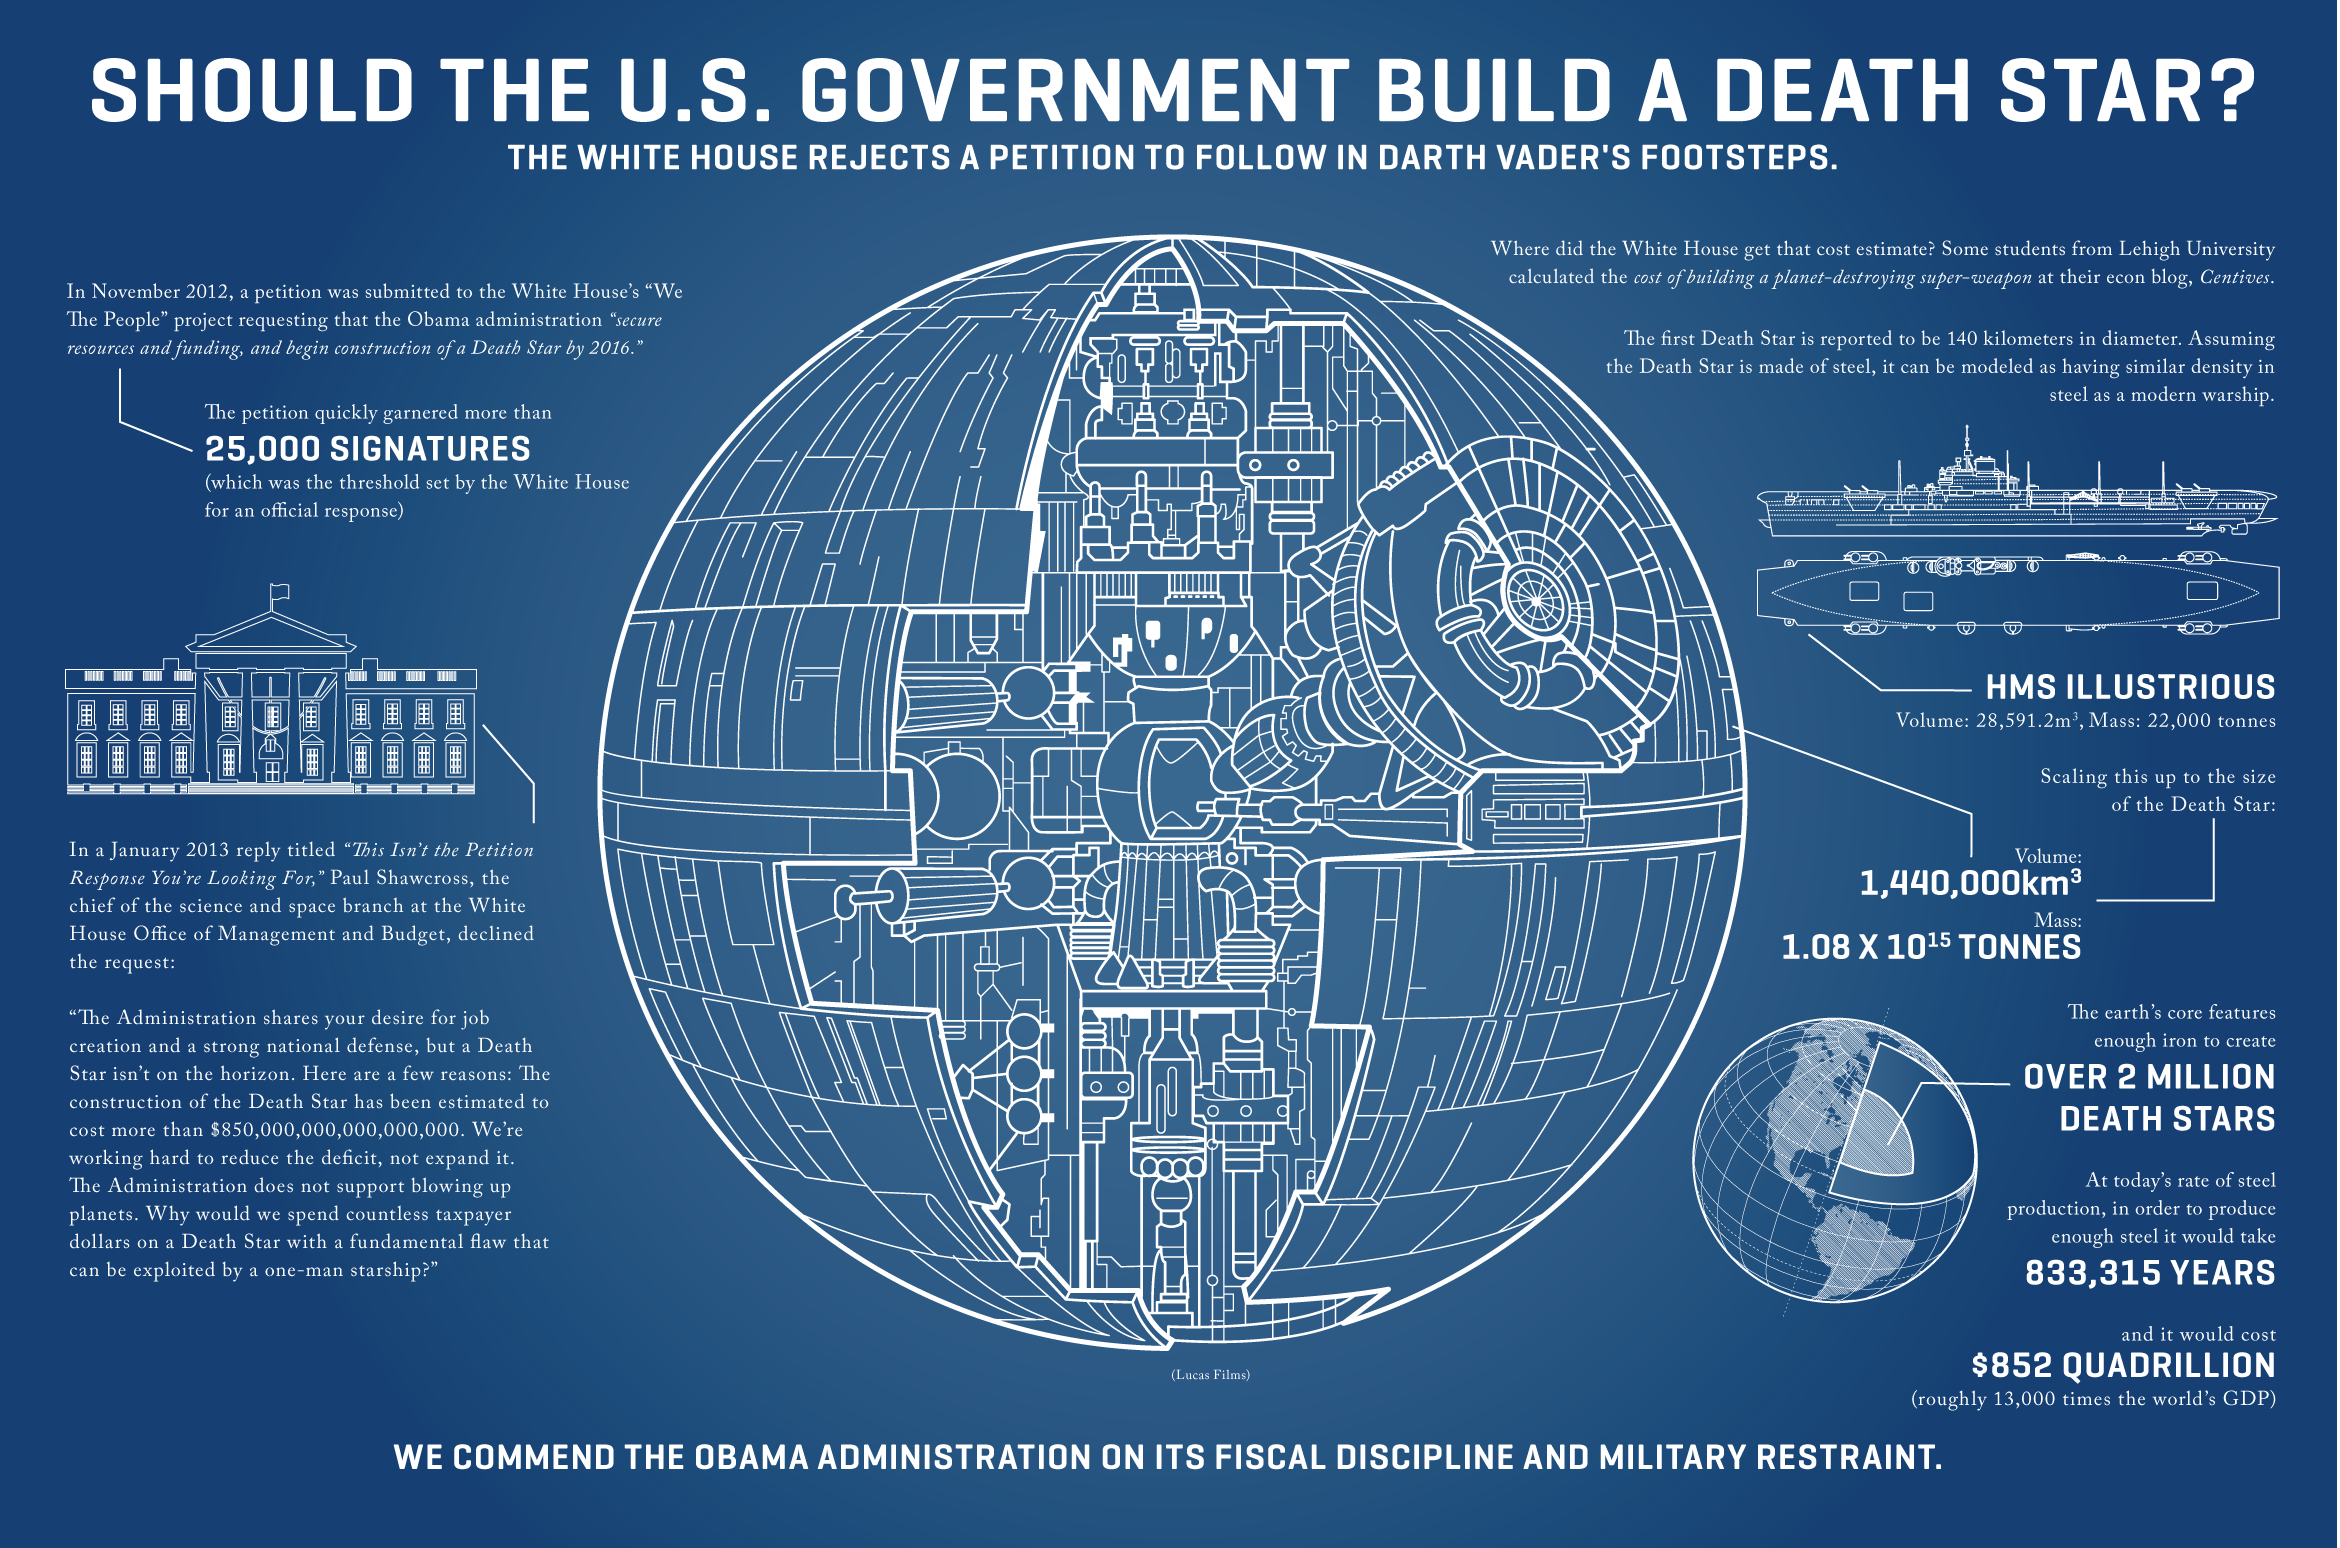
\includegraphics[width=\linewidth]{resources/plans/deathstarinfographic.pNg}
%	\caption{\texttt{deathstarinfographic.pNg}}
%	\label{fig:deathstarinfographic}
%\end{figure}

\end{appendices}
\end{document}
